\documentclass[newpage,hints,handout]{ximera}

%\usepackage{microtype}
%\usepackage{tikz}
\usepackage{tkz-euclide}
%\usetkzobj{all}
\tikzstyle geometryDiagrams=[rounded corners=.5pt,ultra thick,color=blue!50!black]

\usepackage{tikz-cd}

\colorlet{penColor}{blue!50!black} % Color of a curve in a plot

%% \hypersetup{
%%     colorlinks = false,
%%     }


\tikzset{%% partial ellipse
    partial ellipse/.style args={#1:#2:#3}{
        insert path={+ (#1:#3) arc (#1:#2:#3)}
    }
}

\graphicspath{
{./}
{sphericalLunesAndTriangles/}
{hyperbolicLunesAndTriangles/}
{centralProjection/}
{stereographicProjection/}
{linesAnglesAndAreasInCentralProjection/}
{linesAnglesAndAreasInStereographicProjection/}
{stereographicProjection/}
{centralProjectionInHG/}
{stereographicProjectionInHG/}
{linesInSphericalGeometry/}
{linesInHyperbolicGeometry/}
{theArtOfEscher/}
}


\newcommand{\transpose}{\intercal}
\newcommand{\eval}[1]{\bigg[ #1 \bigg]}

\renewcommand{\epsilon}{\varepsilon}
\renewcommand{\l}{\ell}
\renewcommand{\d}{\,d}

\DeclareMathOperator{\arccosh}{arccosh}
\DeclareMathOperator{\arctanh}{arctanh}
\renewcommand{\tilde}{\widetilde}
\newcommand{\R}{\mathbb R}
\newcommand{\dd}[2][]{\frac{d #1}{d #2}}
\newcommand{\pp}[2][]{\frac{\partial #1}{\partial #2}}
\newcommand{\dfn}{\textbf}

\renewcommand{\bar}{\overline}
\renewcommand{\hat}{\widehat}


\ifxake
\NewEnviron{freeResponse}{}
\fi


\setcounter{problem}{107}

\title{Tessellations of the Euclidean plane and Platonic solids}
\begin{document}
\begin{abstract}
In this activity we begin to see the number of equilateral triangles around a point affects geometry.
\end{abstract}
\maketitle
This material was adapted from the Illinois Geometry Labs workshops on tessellations and Platonic solids, the Summer Illinois Math Camp course ``When Straight Lines Curve," and the Buckeye Aha! Math Moments summer 2020 Beyond the Classroom.


We will start by returning to Euclidean geometry. 
\section{Tessellations of the Euclidean plane}
\begin{listOutcomes}
 \item Prove which regular polygons tile the Euclidean plane
\end{listOutcomes}
\begin{definition} 
A \emph{regular polygon }is a polygon where all the edges are the same length and all of the angles are congruent. \end{definition}

\begin{definition} A \emph{tessellation} or \emph{tiling} of a surface is the covering of the surface using one or more geometric shapes, called tiles, with no overlaps and no gaps.An \emph{edge-to-edge tiling} is tessellation with polygonal tiles where adjacent tiles only share one full side, i.e., no tile shares a partial side or more than one side with any other tile. 

A \emph{regular tiling} is an edgge-to-edge tiling where every tile is the same regular polygon and the vertex.
\end{definition}

We will be looking at tilings of the Euclidean plane using regular polygons.


\begin{problem}
\begin{enumerate}
\item In neutral and spherical geometry, we saw that the formula for the sum of the interior angles of an $n$-gon is \[(n-2)*(sum\ of \ the\ interior\ angles\ of\ a\ triangle).\]  This is also true in Euclidean geometry, even though we didn't prove it. Use this fact to write down formula for the the sum of the interior angles of a Euclidean $n$-gon. Your answer should be a formula and nothing else.
\item What is the formula for the measure of one interior angle of a regular $n$-gon? Your answer should be a formula and nothing else.
\end{enumerate}
\end{problem}
\begin{problem}
Now we want to see which regular polygons can be used as tiles for regular tilings. Draw or cut out at least 3 copies of the each regular polygon from the end of this chapter. For some of the smaller shapes, you will need more. You can draw them on paper or a tablet, or you can use the website \url{https://mathigon.org/polypad}

Fill out the following chart:

\begin{tabular}{|p{3cm}|p{1.2cm}|p{2cm}|p{1.5cm}|p{2cm}|}\hline
 Shape & Number of {vertices} & Measure of one interior angle  & Tessellate? & Number that meet at a point\\\hline
 Triangle &&&&\\\hline
 Square&&&&\\\hline
 Pentagon&&&&\\\hline
 Hexagon&&&&\\\hline
 Heptagon&&&&\\\hline
Octagon&&&&\\\hline
 \vdots\\\hline
 $n$-gon&&&&\\\hline
\end{tabular}
\end{problem}
\begin{problem}
 Which regular polygons can be used a tile for a regular tiling? How do you know that you found all of them?
 
\begin{hint}
Argue why number of regular polygons that meet at a vertex must be a positive integer, then explain why you know you have found all possible polygons that can be used as tiles in a regular tessellation. 
\end{hint}
\end{problem}

\section{Platonic solids}
\begin{listOutcomes}
\item Find all Platonic solids.
\item Find a relationship between the faces, vertices, and edges of Platonic solids.
\end{listOutcomes}
If we have less than $360^\circ$ around a point, like if we glued together 5 equilateral triangles, we would get a cone point. 

\begin{definition}
 A \emph{Platonic solid} is a polyhedra where every face is a regular polygon, the adjacent faces share a full side, and the same number of faces meet at each vertex.
\end{definition}

\begin{problem}
\begin{enumerate}
 \item How many Platonic solids can you make with equilateral triangles? 
 \begin{hint} Use Platonic solids have the same number of faces at each vertex, and the Platonic solid with 5 faces at each vertex is different from the solid with four faces at each vertex.
 \end{hint}
 \item How many Platonic solids can you make with squares?
 \item How many Platonic solids can you make with pentagons?
 \item Are there any other Platonic solids?
\end{enumerate}
\end{problem}

\begin{problem}  Now fill out this other table 

\begin{center}
\begin{tabular}{||c|c|c|c||}
\hline 
\hline 
Polyhedra & \# Faces & \# Vertices & \#Edges\\
\hline
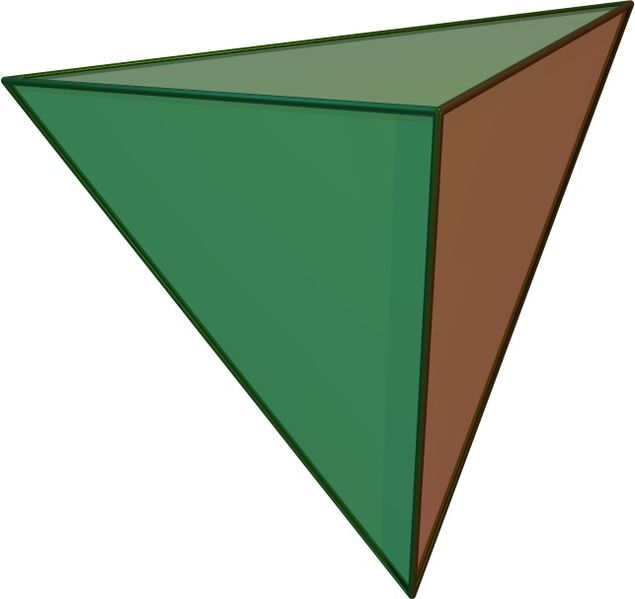
\includegraphics[width=1in]{Tetrahedron} &   &   &  \\\hline
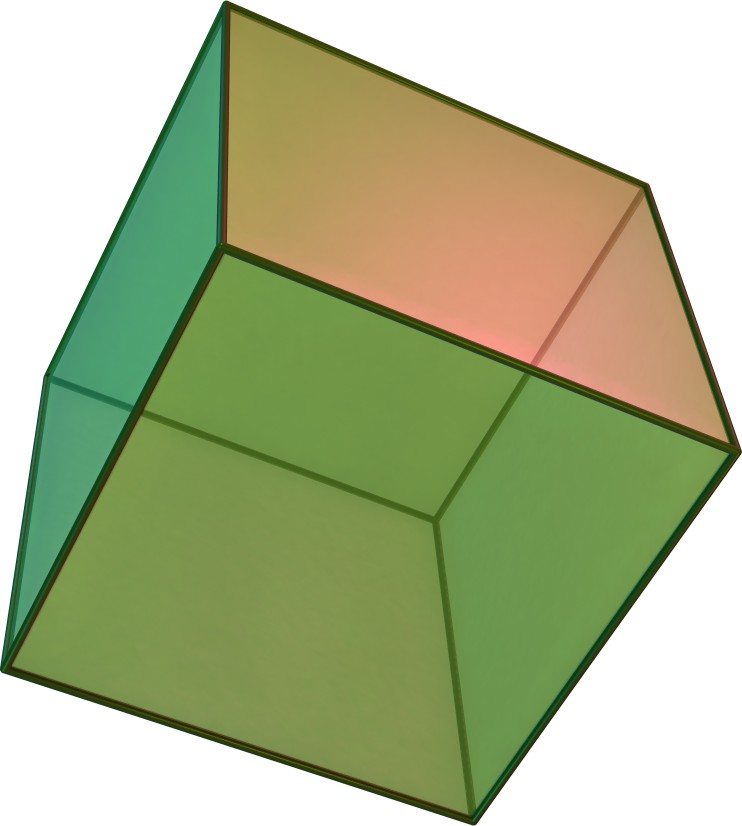
\includegraphics[width=1in]{Hexahedron} &   &   &  \\\hline
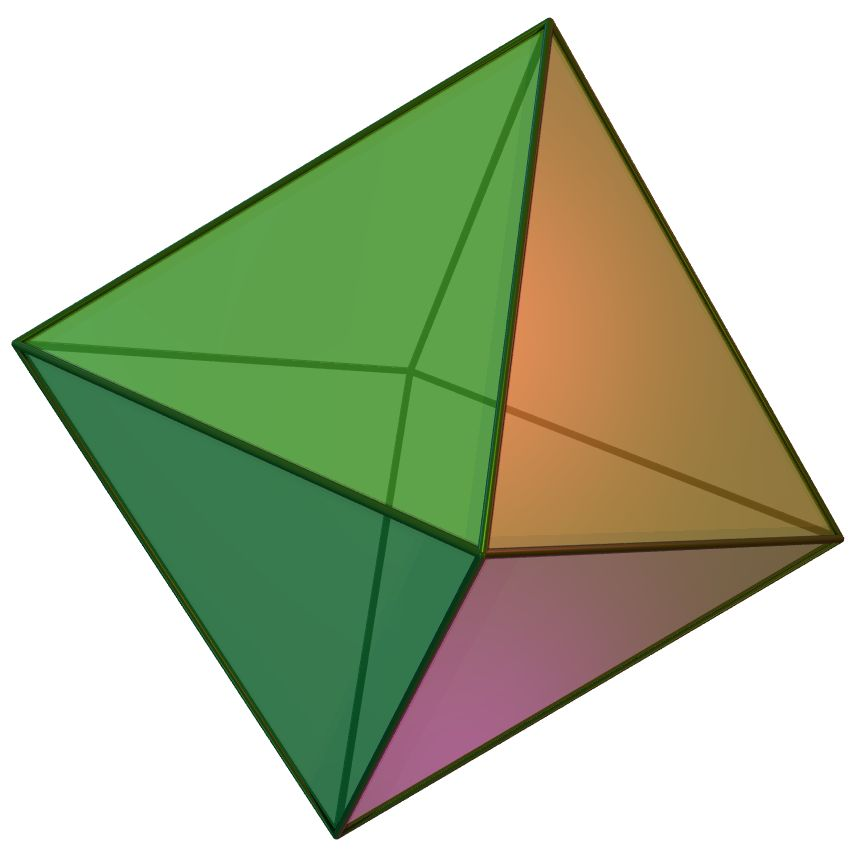
\includegraphics[width=1in]{Octahedron} &   &   &  \\\hline
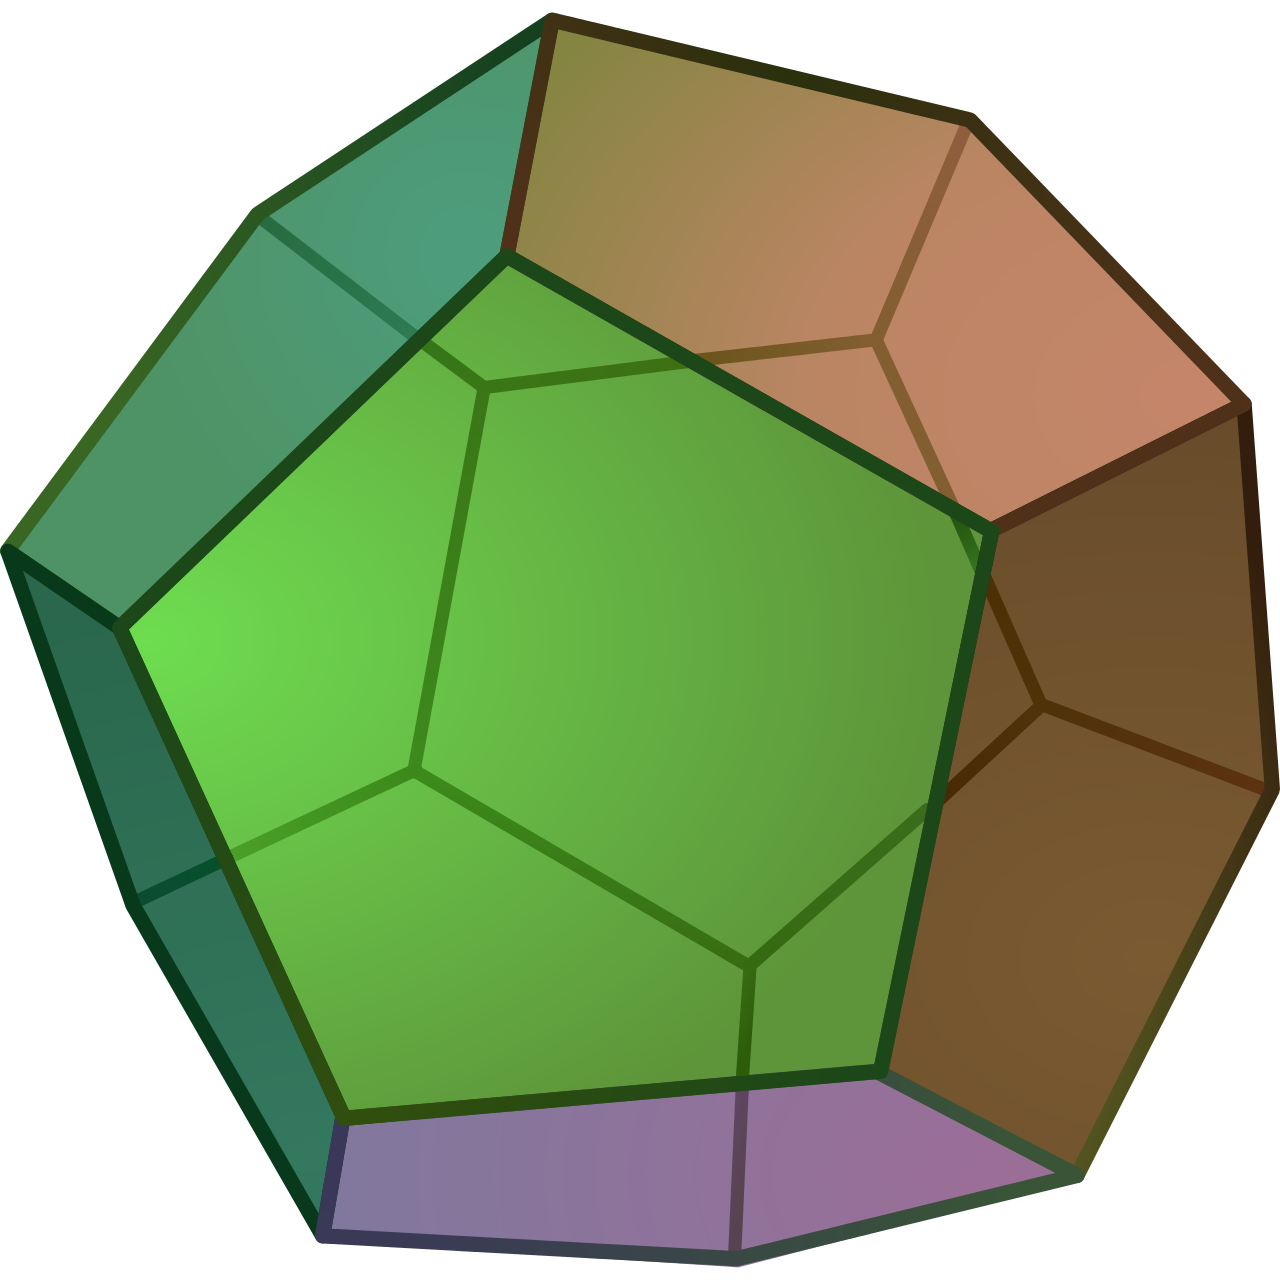
\includegraphics[width=1in]{Dodecahedron} &   &   &  \\\hline
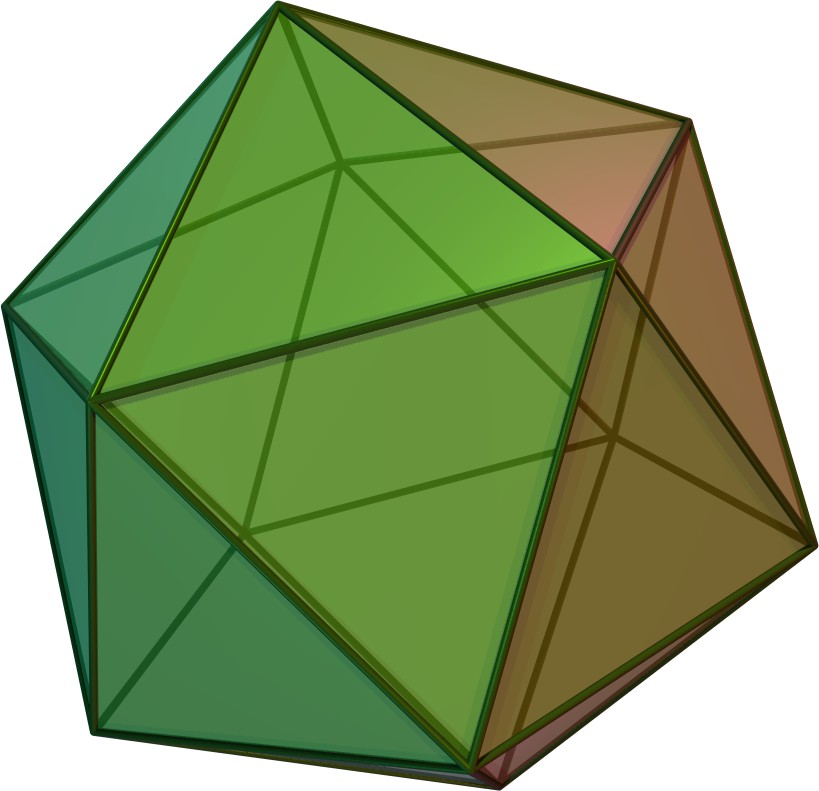
\includegraphics[width=1in]{Icosahedron} &   &   &  \\\hline

\hline
\end{tabular}
\end{center}
Images from \url{https://en.wikipedia.org/wiki/Platonic_solid}
\end{problem}


\begin{problem}
What patterns are in the table above?  Find at least 3 patterns in the table, at least one which describes a relationship between the faces, vertices, and edges.
\end{problem}

\begin{problem}
 Print, trace or draw two copies of the following diagram. You will also need extra equilateral triangle congruent to the ones in the diagram. 
 
\begin{enumerate}
 \item  Cut out one copy and remove triangles so that every vertex is either surrounded by 5 equilateral triangle or is on an edge of the shape. What happens to the paper when you do this?
 \item Cut out one copy and add triangles so that every vertex is either surrounded by 7 equilateral triangle or is on an edge of the shape. What happens to the paper when you do this?
 \item We can think of the shape with 5 triangles at a vertex as having positive curvature. Why? Why would it make sense to also say that the shape with 7 triangles at a vertex has negative curature?
\end{enumerate}
\begin{image}
 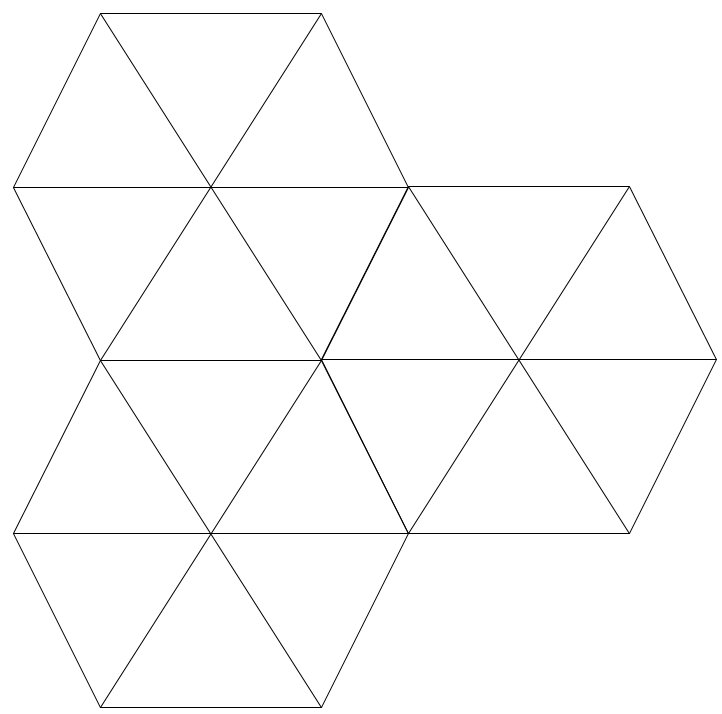
\includegraphics[width=1.5\textwidth]{Hexagons.png}
\end{image}
\end{problem}

\begin{problem}
 Summarize the results from this section. In particular, rephrase the results in your own words and indicate which results follow from the others.
\end{problem}
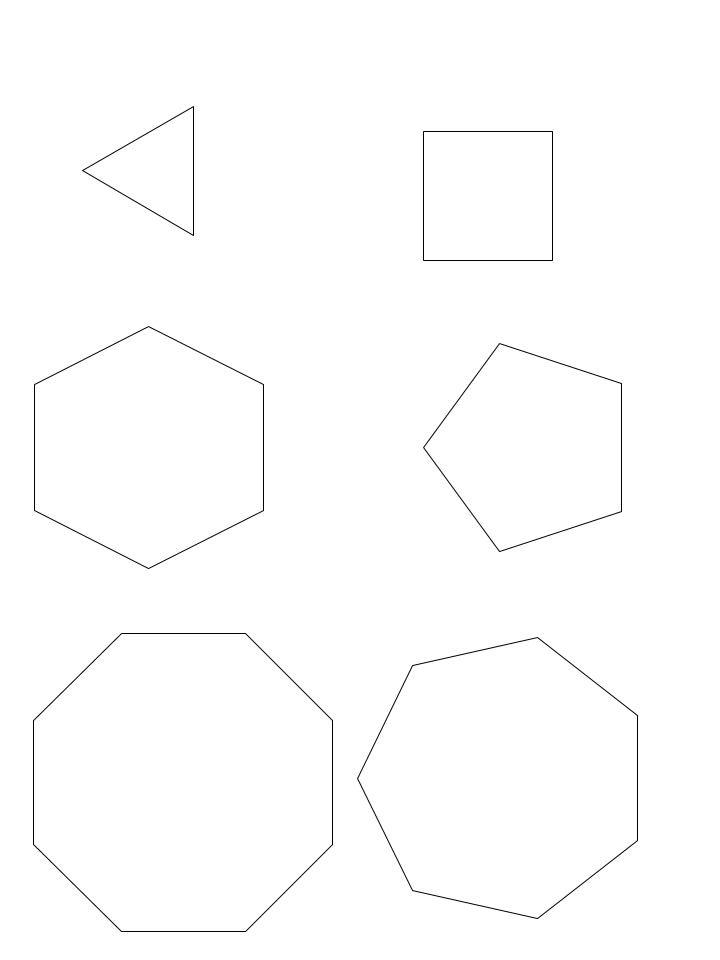
\includegraphics[width=\textwidth]{RegularPolyhedra}
\end{document}